\setRL
\clearpage
\def \MemFluc {\Mempath /MembraneFluc}

\section{
چکیده
}
در این فصل با استفاده از روش تحلیل افت و خیز، انرژی پوسته‌های نازک در حال نوسان را بررسی می‌کنیم. مطالعه‌ی افت و خیز‌های سطحی اطلاعات خوبی راجع به فیزیک حاکم بر سیستم در اختیار مشاهده‌گر قرار می‌دهد. همچنین با استفاده از قضیه‌ی هم پاری انرژی می‌توان شدت‌ مد‌های نوسانی مختلف را پیش‌بینی کرد و حتی مقیاس زمانی نوسانات را تخمین زد.

\section{
مقدمه
}




در فصول قبل نحوه‌ی محاسبه‌ی انرژی انحنا و کششی سطوح دو بعدی را مطالعه کردیم. حال فرض می‌کنیم که یک رویه‌ی دو بعدی با هندسه‌ی بسته در اختیار داریم که حجم کاهیده‌ی آن نزدیک به یک کُره است. سطح این رویه به علت اُفت و خیز ترمودینامیکی محیط دائم در حال تغییر است. در صورتی که یک لحظه زمان را متوقف کنیم، رویه‌ای خواهیم داشت که سطح آن پُر از برآمدگی و فرورفتگی در مکان‌های تصادفی است. اگر فرض کنیم اطلاعات مکانی تمام نقاط روی سطح را در اختیار داشته باشیم چطور می‌توانیم انرژی انحنا یا انرژی کشش این سطح را اندازه‌گیری کنیم؟ 

\begin{figure}[h]
\begin{center}
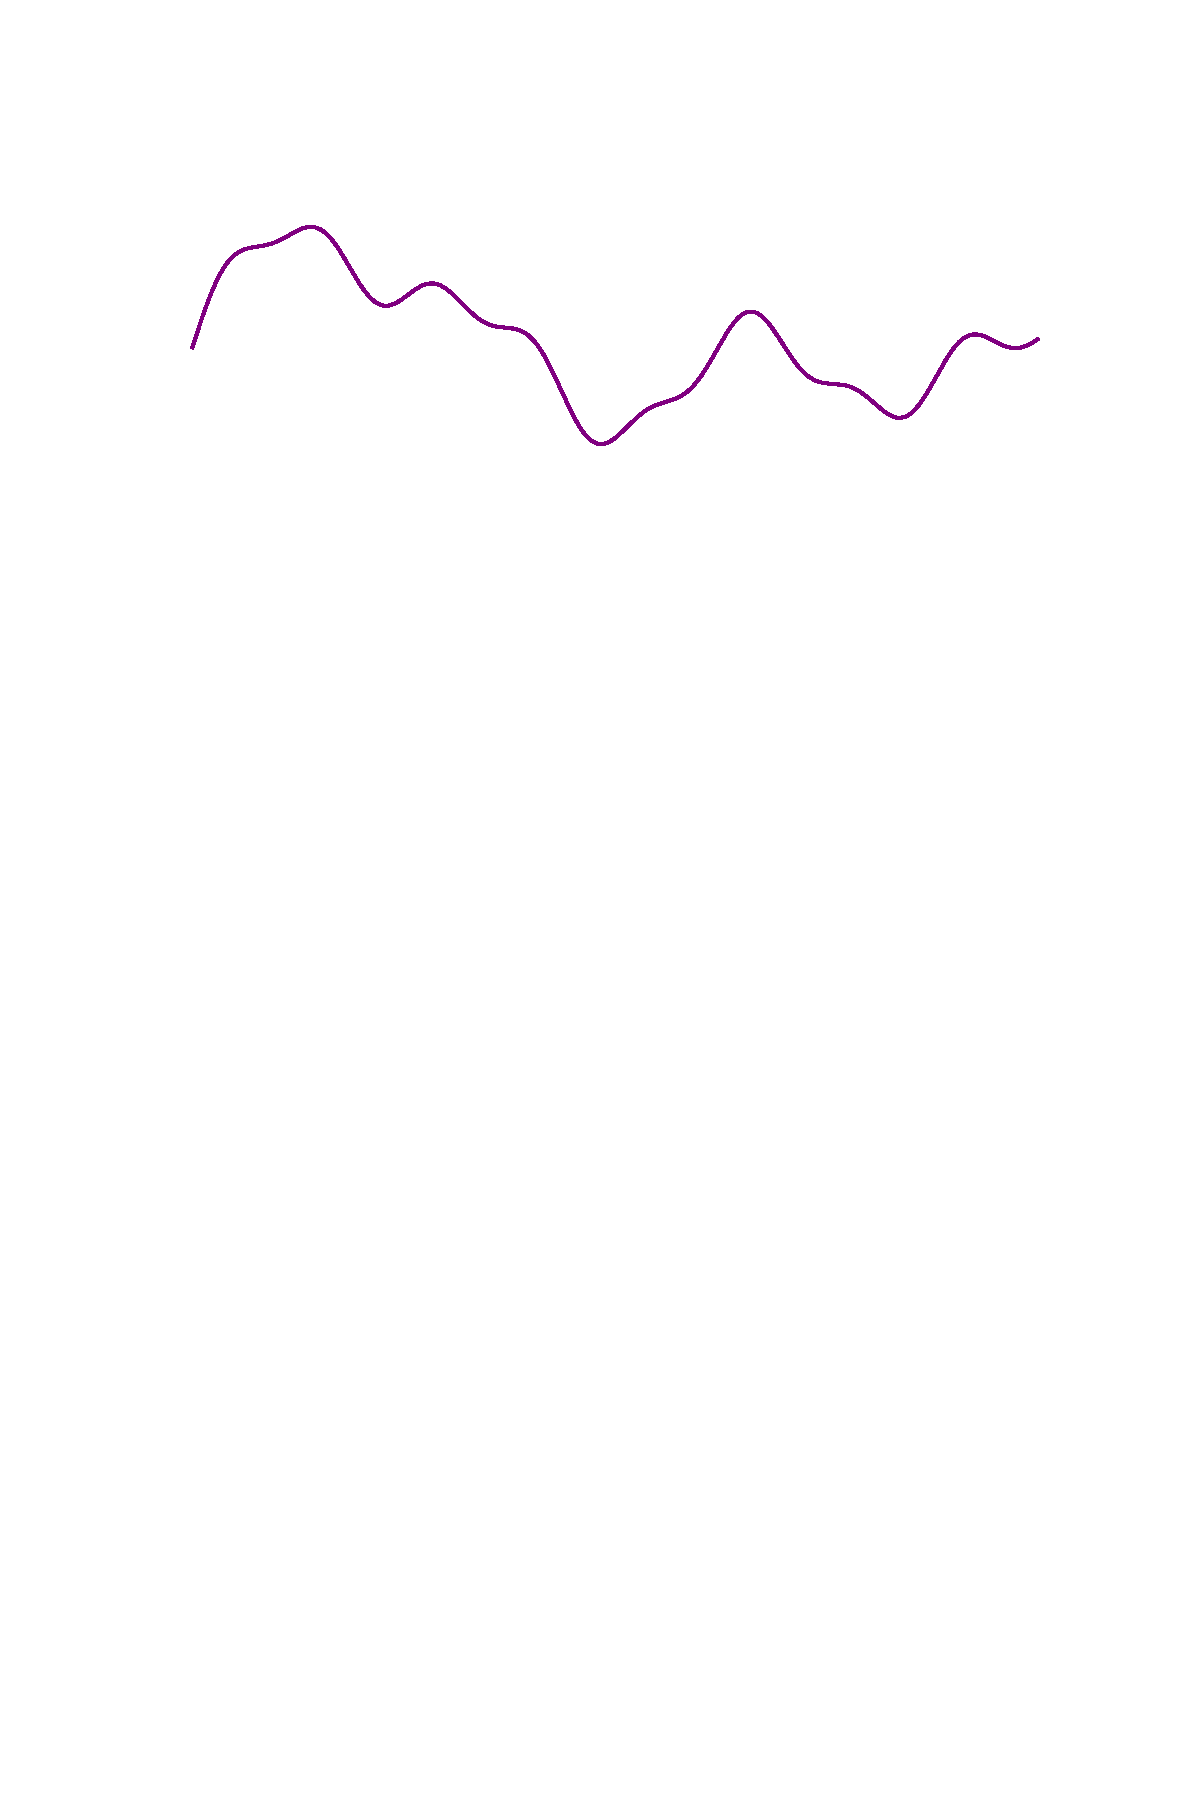
\includegraphics[width=6in]{\MemFluc /Pics/signal_1}
\caption{
 یک ریسمان که در حال افت و خیز در فضای ۲ بعدی. دو انتهای ریسمان ثابت است.
}
\label{fig:flucString1}
\end{center}
\end{figure}


حالا فرض کنیم که مسئله‌ی ساده‌تری را مطالعه می‌کنیم. فرض کنیم که به جای رویه، یک ریسمان در اختیار داریم که دو سر آن ثابت است و ریسمان  در یک فضای ۲ بعدی  در حال افت و خیز است. در شکل 
\ref{fig:flucString1}
چیدمان این ریسمان در زمان تصادفی‌ رسم شده‌است.
\begin{figure}[h]
\begin{center}
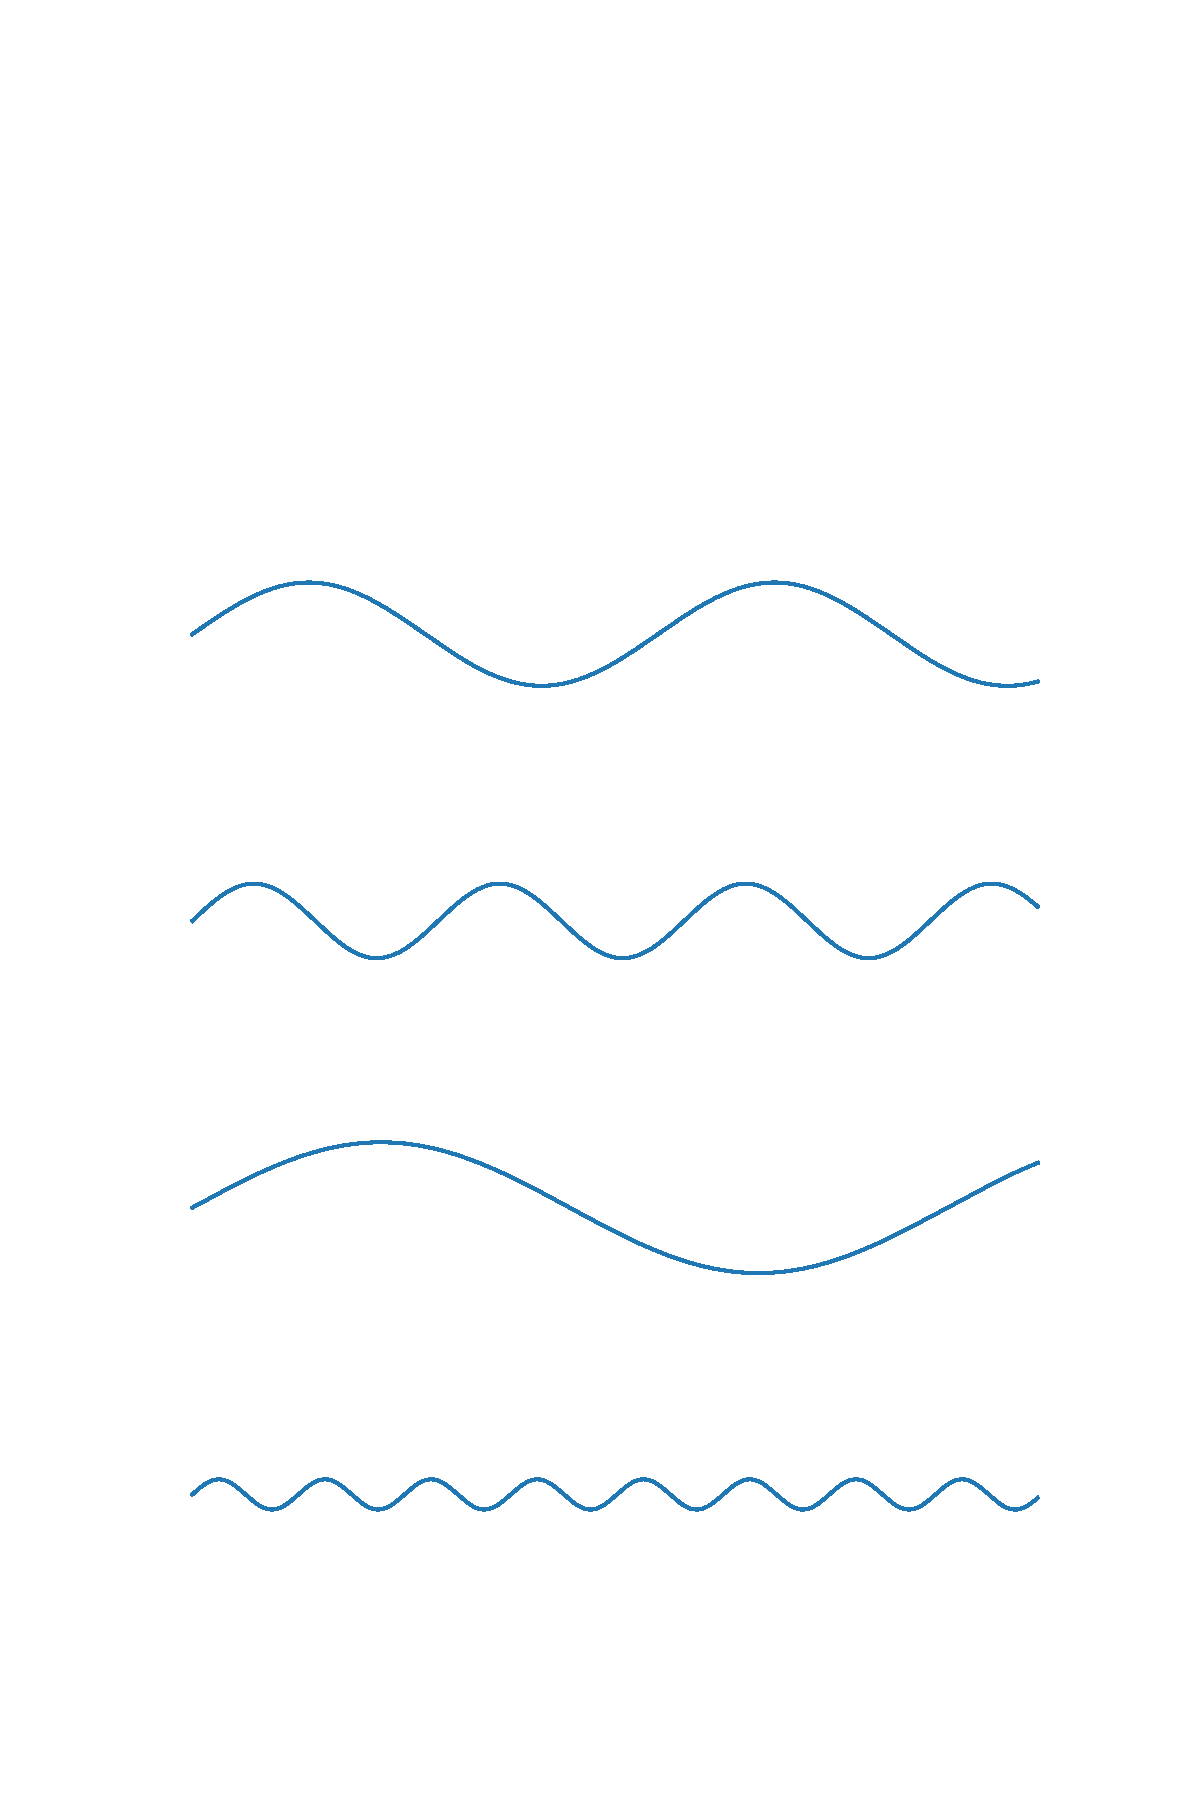
\includegraphics[width=4in]{\MemFluc /Pics/signal_2}
\caption{
مُدهای نرمال تشکیل دهنده‌ی شکل
\ref{fig:flucString1}
را نشان می‌دهد. شکل
\ref{fig:flucString1}
از چهار مُد نرمال با فرکانس و شد‌ت مختلف ساخته شده‌است. 
}
\label{fig:flucString2}
\end{center}
\end{figure}
در صورتی که لازم باشد اطلاعات ساده‌ای مانند انرژی جنبشی یا انرژی پتانسیل این ریسمان محاسبه شود، با فرض اینکه اصل برهم نهی بر قرار است، کافی است که مُدهای نرمال این ریسمان را پیدا کنیم. مُدهای نرمال این ریسمان با توابع مثلثاتی تعریف می‌شوند. با محاسبه‌ی مجموع انرژی جنبشی یا پتانیسل مُدهای تشکیل دهنده‌ی این شکل می‌توانیم انرژی کلی جنبشی یا پتانسیل این ریسمان را محاسبه کنیم. در شکل
\ref{fig:flucString2}
مد‌های تشیل دهنده‌ی این ریسمان رسم شده‌است.


.
 
 
 
 
 
 
 
 
 
 
 

\section{
محاسبه‌ی اندازه افت و خیز روی کره
\label{sec:bendingFluctuations}
}
\input{\MemFluc/spherical}

\section{
افت و خیز مساحت و حجم کُره
}

 کُره‌ بر اساس تعریف آن حجم کاهیده‌ی 
 $\nu=1$
 دارد. غشا با حجم کاهیده‌ی واحد نمی‌تواند افت و خیز کند، زیراکه برای افت و خیز مساحت آن باید کمی بیشتر از مساحت کُره با همان حجم باشد. می‌توانیم مساحت شکلی که در حال افت و خیز است را به شکل زیر محاسبه کنیم. از بخش قبل می‌دانیم که
\begin{equation}
dA=r_{0}^2(1+g^2+\frac{1}{2}g\mathcal{L}^2g)d\Omega
\label{eq:areaPatchDifferential}
\end{equation}
 و با انتگرال گیری روی تمام زوایای فضایی،
 \begin{equation}
\begin{aligned}
A&=\int dA=r_{0}^2\int(1+g^2+\frac{1}{2}g\mathcal{L}^2g)d\Omega\\
&=r_{0}^2(4\pi+\sum_{\ell}|u_{\ell,m}|^2[1+\frac{1}{2}\ell(\ell+1)])
\label{eq:AreaGL}
\end{aligned}
\end{equation}
 حجم غشای در حال افت و خیز نیز به همین ترتیب قابل محاسبه‌است. با انتگرال گیری بر روی تمام زوایای فضای حجم غشا را محاسبه می‌کنیم،
\begin{equation}
\begin{aligned}
V&=\int dV=\frac{1}{3}\int r^3d\Omega\\
&=\frac{1}{3}r_{0}^3\int(1+g)^3d\Omega=\frac{1}{3}r_{0}^3\int1+3g+3g^2d\Omega\\
&=\frac{1}{3}r_{0}^3(4\pi+3\sum_{\ell}|u_{\ell,m}|^2)
\label{eq:VolumeGL}
\end{aligned}
\end{equation}
حالا با استفاده از معادلات
\ref{eq:AreaGL}
و
\ref{eq:VolumeGL}
و جایگذاری در معادله‌ی
\ref{eq:reducedVolume}
حجم کاهیده شکل در حال افت و خیز  را محاسبه می‌کنیم،
\begin{equation}
\begin{aligned}
\nu=\frac{\sqrt{4\pi}(4\pi+\sum|u_{\ell,m}|^2)}{(4\pi+3\sum|u_{\ell,m}|^2[1+\frac{1}{2}\ell(\ell+1)])^{3/2}}
\label{eq:nuUndulated}
\end{aligned}
\end{equation}
%با فرض اینکه ضریب سختی خمش یک غشا حدود
%$\kappa=20k_BT$
%است، با جمع روی مُدها می‌توان حجم کاهیده‌ی لازم را حدود
%$\nu\approx0.9626$
%تخمین زد.


\section{
افت و خیز سطح کُره‌ی جامد
}
کانون توجه این رساله بررسی اُفت و خیز سطح غشا‌های جامد (مانند شبکه‌ی پلیمری گلبول‌های قرمز) و پوسته‌های الاستیکی

نیست. اما جهت تکمیل مطالعه‌ی افت و خیز، لازم می‌دانم که به شکل شدت افت و خیز سطح پوسته‌ی کروی الاستیک به شعاع
$R$
، مدول یانگ دو بعدی
$Y_{2d}$
، خمش ذاتی 
$r_s=R$
، سختی خمش
$\kappa$
، و تحت اختلاف فشار 
$p$
در دمای 
$k_BT$
را معرفی کنم. افت و خیز چنین سطحی تا مرتبه‌ی دوم به شکل 
\begin{equation}
\langle|u_{\ell,m}|^2\rangle=\frac{k_BT}{\kappa(\ell+2)^2(\ell-1)^2-pR^3\left[1+\frac{1}{2}\ell(\ell+1)\right]+R^2\frac{Y_{2D}}{1+\frac{Y_{2D}}{2\mu(\ell^2+\ell-2)}}}
\label{eq:ulmSolid}
\end{equation}


تعریف می‌شود. و تعریف مدول یانگ دو بعدی بر حسب ضرایب لمه
\LTRfootnote{lam\'e coefficients}
$\lambda,\mu$
به شکل
\begin{equation}
Y_{2D}=\frac{4\mu(\mu+\lambda)}{2\mu+\lambda}
\label{eq:youngLame}
\end{equation}

است. همچنین می‌توان معادله‌ی
\ref{eq:ulmSolid}
را برای ماده‌ای که دارای تنش بُرشی 
$\mu=3Y_{2D}/8$
باشد (مثلا موادی که اتصالاتشان شبکه‌ی مثلثی تشکیل می‌دهد) به شکل زیر تقریب زد،
\begin{equation}
\langle|u_{\ell,m}|^2\rangle=\frac{k_BT}{\kappa(\ell+2)^2(\ell-1)^2-pR^3\left[1+\frac{1}{2}\ell(\ell+1)\right]+Y_{2D}R^2\frac{3(\ell^2+\ell-2)}{3(\ell^2+\ell)-2}}
\label{eq:ulmSolidTri}
\end{equation}
جزئیات محاسبات بخش خمش طبق محاسبات ارائه شده در این رساله‌است و محاسبات مربوط به اثر فشار و خاصیت الاستیکی سطح با جزئیات کامل در مرجع
\cite{gomppernelson2012}
یافت می‌شود.


\section{
افت و خیز بر روی مدارهای
$\theta$
}




در بخش‌های قبل اطلاعات دامنه‌ی افت و خیز کره (مد‌های هماهنگ کروی بر رویه‌ی ۲ بعدی در فضای ۳ بعدیی) را محاسبه‌ کردیم. برای اندازه‌گیری شدت دامنه‌ی مد‌های بر برش‌های در راستای 
$\theta$
(مد‌های هماهنگ بر حلقه‌ی ۱ بعدی در فضای ۲ بعدی) کافی‌است که  تصویر همه‌ی مد‌ها را در بُرش مورد نظر جمع بزنیم
\cite{Prost2004}
.
\begin{equation}
\langle|u_m(\theta)|^2\rangle=\sum_{\ell=m}^{\ell=\ell_{max}}\frac{2\ell+1}{4\pi}\frac{(\ell-|m|)!}{(\ell+|m|)!}\left(P_\ell^{|m|}(\cos(\theta))\right)^2\langle|u_{\ell,m}|^2\rangle
\label{eq:3Dto2Dsum}
\end{equation}


\section{
مقیاس زمانی
}

در این بخش به محاسبه‌ی زمان دوره‌ی تناوبی بسامد نوسان‌‌های هماهنگ‌های کروی برای یک غشای سیال‌گون می‌پردازیم. 
در بخش 
\ref{sec:bendingFluctuations}
انرژی انحنای یک غشای بر اساس مُدهای نرمال آن (هماهنگ‌های کُروی) محاسبه شد. معادله‌ی لاگرانژ، دینامیک درجه‌های آزادی را به تغییرات انرژی درجات آزادی، 
$q$
مرتبط می‌کند،

\begin{equation}
\frac{d}{dt}\left(\frac{\partial K}{\partial \dot q}\right)=-\frac{\partial U}{\partial q}.
\label{eq:LagrangeEquation}
\end{equation}
در معادله‌ی فوق
$K$
انرژی جنبشی،
$U$
انرژی پتانسیل سیستم مورد مطالعه‌است. این معادله مستقل از شکل معادله‌ی دینامیک سیستم بر قرار است. در صورتی که غشا در محیط خلا در حال نوسان باشد، معادله‌ی حرکت سیستم توسط معادله‌ی نیوتن تعیین می‌شود. در صورتی که غشا در محیط سیال در حال نوسان باشد، معادله‌ی حرکت با حل معادله‌ی ناویر-استوکس
\LTRfootnote{Navier-Stokes }
تعیین می‌شود. برای غشایی که در خلا حرکت می‌کند، انرژی جنبشی آن به سادگی با جمع روی انرژی جنبشی تکه‌های جرمی کوچک برای سطح آن محاسبه می‌شود،
\begin{equation}
\begin{aligned}
K&=\frac{1}{2}\rho_m\int\d\Omega~\dot r^2(\theta,\phi) dm=\frac{1}{2} \left\{\frac{\partial}{\partial t}\left[r_0(1+\sum_{\ell,m}u_{\ell,m}Y_{\ell,m})\right\}\right)^2\\
&=\frac{1}{2} \rho_mr_0^2\int d\Omega\left[\sum_{\ell,m}\frac{\partial}{\partial t}u_{\ell,m}Y_{\ell,m}\right]^2\\
&=\frac{1}{2} \rho_mr_0^2\sum_{\ell,m}\dot u_{\ell,m}^2
\end{aligned}
\label{eq:kineticEnergyNewton}
\end{equation}
در محاسبات فوق فرض شده که غشایی به جرم 
$M$
با چگالی یکنواخت در تمام جهت فضا 
$\rho_m=M/4\pi$
در حال حرکت است. حالا می‌توانیم معادله‌ی لاگرانژ را برای یک غشای در حال نوسان در خلا محاسبه کنیم،
\begin{equation}
\begin{aligned}
\frac{d}{dt}\left(\frac{\partial}{\partial \dot u_{\ell,m}}\frac{1}{2}\frac{Mr_0^2}{4\pi}\sum_{\ell',m'}\dot u_{\ell',m'}^2\right)&=-\frac{\partial}{\partial u_{\ell,m}}\left[ 8\pi\kappa +\frac{1}{2}\kappa\sum_{\ell',m'}|u_{\ell',m'}|^2(\ell'+2)(\ell'+1)\ell'(\ell'-1)\right]\\
\frac{Mr_0^2}{4\pi}\ddot u_{\ell,m}&=-\kappa u_{\ell,m}(\ell+2)(\ell+1)\ell(\ell-1)\\
\ddot u_{\ell,m}&=-\frac{4\pi\kappa}{Mr_0^2}(\ell+2)(\ell+1)\ell(\ell-1)~u_{\ell,m}
\end{aligned}
\label{eq:LagrangeNewton}
\end{equation}
که شکل معادله‌ی نوسانگر هارمونیک را دارد. در نتیجه بسامد زاویه‌ای هر مُد برابر با،
\begin{equation}
\omega_{\ell,m}^2=\frac{4\pi\kappa}{Mr_0^2}(\ell+2)(\ell+1)\ell(\ell-1)
\label{eq:Omegalm}
\end{equation}
است. در نتیجه مقیاس زمانی برای نوسان هر مُد مشخص شده‌است. رابطه‌ی 
$\omega_{\ell,m}$
و
$\ell$
یک رابطه‌ی مستقیم است، یعنی مُدهای بالا بسامد بزرگتری خواهند داشت. با توجه به اینکه 
\begin{equation}
T=\frac{2\pi}{\omega}
\end{equation}

کوچکترین مُد سیستم که تغییر شکل ایجاد می‌کند،
$\ell=2$
طولانی ترین دوره‌ی تناوب را دارد و هر جه مُد بالاتر باشد، دوره‌ی تنواب سریع‌تری خواهد داشت.
\begin{equation}
T_{\ell,m}=\sqrt{\frac{M\pi r_0^2}{\kappa}\frac{1}{(\ell+2)(\ell+1)\ell(\ell-1)}}
\end{equation}
این نکته‌ی کلیدی در انتخاب قدم زمانی مناسب برای پیاده‌سازی محاسبات دینامیک ملکولی است.

جهت تکمیل کردن بحث، انرژی جنبشی سطح غشا بین دو سیال تراکم ناپذیر با چگالی 
$\rho_1$
(سیال داخل غشا) و 
$\rho_2$
شکل زیر را خواهد داشت،
\cite{Christer1984}
\begin{equation}
K=\frac{1}{2}r_0^5\sum_{\ell,m}\left(\frac{\rho_1}{\ell}+\frac{\rho_2}{\ell+1}\right)\dot u_{\ell,m}^2
\end{equation}
که با حل معادله ناویر-استکس به دست می‌آید.














